\documentclass[a4paper, 12pt]{article}
\usepackage[utf8]{inputenc}
\usepackage{graphicx} % Required for inserting images
% pacote acentuação
\usepackage[brazil]{babel}
\usepackage[lmargin=3cm, tmargin=3cm, rmargin=2cm, bmargin=2cm]{geometry}
\usepackage[T1]{fontenc} %ajusta o texto que vem de outras fontes
\usepackage{blindtext}
\usepackage{setspace}
\usepackage{indentfirst}

\usepackage[export]{adjustbox}
% Agora você pode usar \includegraphics[width=0.8\textwidth, keepaspectratio]{imagem.png}
\setlength{\parindent}{1.25cm}
\onehalfspacing % Define espaçamento 1.5 para o documento todo


\title{Projeto APO2 - HelpDesk}

\author{Dandara Santos de Almeida}
\author{Rayssa Soares Oliveira Azevedo}
\date{April 2026}

\begin{document}
\pagenumbering{gobble} % Desativa a numeração

% Capa
\begin{titlepage}
    \begin{center}
        % Nome da Instituição
        \Large\textbf{INSTITUTO FEDERAL DE EDUCAÇÃO, CIÊNCIA E TECNOLOGIA DE SÃO PAULO}\\[2cm]
        
        \large\textbf{BACHARELADO EM ENGENHARIA COMPUTAÇÃO}\\[4cm]

        % Título do Projeto
        \LARGE\textbf{SISTEMA DE HELP DESK}\\
        \large\textbf{PROJETO DE APO2}\\[2cm]

        % Autores
        \large\textbf{RAYSSA SOARES OLIVEIRA AZEVEDO}\\
        \large\textbf{DANDARA SANTOS DE ALMEIDA}\\[5cm]

        % Local e Data
        \vfill % Empurra o texto para baixo
        \large\textbf{Guarulhos - SP}\\
        \large\textbf{Julho de 2026}
    \end{center}
    \thispagestyle{empty} % Remove o número desta página apenas

\end{titlepage}




\newpage  % OBJEITVOS DO SISTEMA 

\pagenumbering{arabic} % Reativa a numeração e reseta para 1
\section{Objetivos do Sistema}

Fornecer uma plataforma web para abertura, triagem, atendimento e gerenciamento global de chamados de suporte técnico (Help Desk). O sistema visa estruturar a comunicação por meio de três perfis de acesso: Clientes, que registram suas solicitações; Equipe Técnica, que recebe e atende de forma segmentada os chamados correspondentes às suas áreas de especialidade (como hardware, software e redes); e Administradores, que possuem controle irrestrito para o gerenciamento de permissões de usuários, parametrização do sistema e auditoria global de todos os tickets.


\newpage  %EQUIPE E FUNÇÕES
\section{Equipe e Funções dos Integrantes}

Dandara: Responsável pela infraestrutura do Banco de Dados (scripts DDL/DML), elaboração dos diagramas UML (Diagrama de Classes e Diagrama Entidade-Relacionamento) e desenvolvimento frontend do sistema,  elaboração da documentação dos testes de endpoint.

Rayssa: Responsável pela análise de requisitos, elaboração dos diagramas de casos de uso e de sequências, desenvolvimento backend, debug e testes de endpoint, elaboração da documentação do sistema em LaTeX.

\newpage    % REQUISITOS FUNCIONAIS
\section{Requisitos Funcionais}
\subsection{ÁREA PÚBLICA (ACESSO LIVRE)}
Esta área concentra as funcionalidades disponíveis para qualquer visitante não autenticado.
\begin{itemize}
    \item \textbf{Acesso à Página Inicial:} O sistema deve apresentar uma landing page com informações sobre o serviço de suporte técnico e botões de acesso rápido.
    \item \textbf{Cadastro de Usuário:} O sistema deve permitir que visitantes se cadastrem informando nome, e-mail e senha.
    \item \textbf{Autenticação de Usuário (Login):} O sistema deve possuir uma tela de login validando o e-mail e a senha no banco de dados.
    \item \textbf{Validação de Cadastro por E-mail:} Após o envio do formulário de cadastro, o sistema deve disparar um e-mail de confirmação *utilizando a ferramenta Mailtrap.
    \item \textbf{Recuperação de Senha:} O sistema deve possuir uma tela para que o usuário informe seu e-mail e receba instruções *(via Mailtrap) para redefinir sua senha esquecida.
\end{itemize}

\subsection{ÁREA PRIVADA DO USUÁRIO}
Esta área é restrita a usuários com perfil de "Cliente" logados no sistema.
    \begin{itemize}
        \item \textbf{Atualização de Dados do Usuário:} O sistema deve disponibilizar uma tela onde o usuário logado possa editar suas próprias informações pessoais (nome, e-mail, senha).
        \item \textbf{Abertura de Chamado:} O sistema deve possuir um formulário para o cliente registrar um novo ticket de suporte, selecionando a categoria do problema e detalhando a ocorrência.
        \item \textbf{Consulta de Meus Chamados:} O sistema deve listar em uma tabela (grid) todos os chamados abertos exclusivamente por aquele usuário, exibindo o status atualizado de cada um.
        \item \textbf{Cancelamento de Chamado:} O sistema deve permitir que o cliente encerre um chamado aberto por ele mesmo, caso o problema tenha sido resolvido antes do atendimento técnico.
    \end{itemize}

\subsection{ÁREA PRIVADA DA EQUIPE TÉCNICA (SUPORTE)}
Esta área concentra as funcionalidades disponíveis para os usuários que compõem a equipe técnica, de acordo com os seus níveis de suporte (hardware, software, redes, etc)
    \begin{itemize}
        \item \textbf{Atualização de Dados do usuário:} O sistema deve permitir que o membro da equipe técnica atualize seus próprios dados de acesso.
        \item  \textbf{Fila de Chamados por Especialidade:} O sistema deve exibir para o técnico apenas os chamados que pertencem às categorias para as quais ele tem permissão de atendimento (ex: O técnico de "Redes" não enxerga a fila de "Software", a menos que tenha ambas as permissões).
        \item \textbf{Resolução e Atualização de Status:}  O sistema deve permitir que o administrador abra os detalhes de um chamado e altere seu status (de "Aberto" para "Em Andamento", "Resolvido", etc.).
        \item \textbf{Redirecionamento de Chamado:} O técnico deve conseguir alterar a categoria de um chamado caso identifique que o problema pertence a outra equipe (ex: um problema relatado como "Software" era, na verdade, "Hardware").
    \end{itemize}

\subsection{ÁREA ADMINISTRATIVA}
Esta área é de acesso exclusivo aos usuários com perfil de "Administrador".
\begin{itemize}
        \item \textbf{Atualização de Dados do Administrador:} O administrador deve poder alterar seus próprios dados de acesso.
        \item \textbf{Gestão Global de Chamados:} O sistema deve exibir um painel listando todos os chamados de todos os clientes, permitindo filtros rápidos (ex: ver apenas os "Abertos").
        \item \textbf{Resolução e Atualização de Status:}  O sistema deve permitir que o administrador abra os detalhes de um chamado e altere seu status (de "Aberto" para "Em Andamento", "Resolvido", etc.).
        \item \textbf{Controle de Acesso e Níveis de Usuários:}  O sistema deve listar todos os usuários cadastrados e permitir que o administrador altere os perfis de acesso (cliente, suporte ou admin).
        \item \textbf{Atribuição de Especialidades:} O administrador deve poder vincular quais categorias de atendimento cada usuário do perfil "Suporte" está autorizado a acessar.
        \item \textbf{Configurações de Categorias:} O sistema deve possuir uma tela para o cadastro, edição e exclusão de Categorias de Suporte, que irão alimentar o formulário de abertura de chamados.
    \end{itemize}

\newpage
\section{Requisitos Não Funcionais}


\begin{itemize}
    \item \textbf{Plataforma e Servidor:} O sistema deve ser desenvolvido na Plataforma J2EE (Jakarta EE) e executado no servidor de aplicação Apache Tomcat, versão 9.0 ou superior.

    \item \textbf{Persistência de Dados:} O armazenamento das informações deve ser realizado de forma relacional utilizando o SGBD MySQL Server, versão 8.0 ou superior.

    \item \textbf{Arquitetura de Software:} O projeto deve adotar o padrão arquitetural MVC (Model-View-Controller) para separar a lógica de negócio, as regras de roteamento (Servlets) e a interface do usuário.

    \item \textbf{Interface de Usuário (Front-end):} As views devem ser construídas utilizando a tecnologia JSP (JavaServer Pages), aplicando o framework Bootstrap 5.0 para garantir a responsividade e estilização da interface.

    \item \textbf{Comunicação Assíncrona:} O sistema deve realizar requisições assíncronas no front-end utilizando a biblioteca jQuery (AJAX), atualizando partes da tela sem a necessidade de recarregar a página inteira.

    \item \textbf{Formato de Intercâmbio de Dados:} Os endpoints desenvolvidos (Servlets) devem obrigatoriamente retornar as respostas das requisições AJAX no formato JSON.

    \item \textbf{Ferramenta de E-mail:} O envio de e-mails para validação de cadastro ou recuperação de senha deve ser simulado/integrado utilizando a ferramenta Mailtrap.
\end{itemize}

\newpage
\section{Histórias de Usuário (User Stories)}
\subsection{Acesso Livre}
    
    Como um visitante, quero criar uma conta informando meus dados básicos para poder solicitar suporte técnico.
    
    Como um usuário, quero solicitar a recuperação da minha senha informando meu e-mail para que eu possa recuperar o acesso à plataforma.
    
    Como um usuário cadastrado, quero fazer login com minhas credenciais para ser direcionado ao meu painel correspondente (Cliente, Suporte ou Admin).

\subsection{Cliente}
    Como cliente, quero abrir um chamado descrevendo meu problema e selecionando a categoria correspondente para receber assistência especializada.

    Como cliente, quero visualizar a lista dos chamados que eu abri para acompanhar o status e o andamento de cada solicitação.

    Como cliente, quero cancelar um chamado que eu abri caso o problema tenha sido resolvido por conta própria, evitando o trabalho desnecessário da equipe.

    Como cliente, quero atualizar meus dados cadastrais e senha para manter meu perfil em dia.

\subsection{Suporte}
    Como técnico de suporte, quero visualizar apenas a fila de chamados das categorias em que sou especialista (ex: Redes) para focar nas demandas da minha área.

    Como técnico de suporte, quero alterar o status de um chamado (ex: de "Aberto" para "Em Andamento" ou "Resolvido") e adicionar observações para registrar o progresso do atendimento.

    Como técnico de suporte, quero alterar a categoria de um chamado caso o cliente tenha classificado errado, para que o ticket seja redirecionado à equipe correta.

    Como técnico de suporte, quero atualizar minhas credenciais de acesso para manter minha conta segura.

\subsection{Administrador}
    Como administrador, quero visualizar todos os chamados registrados no sistema, independentemente da categoria, para auditar o volume de trabalho e identificar gargalos.

    Como administrador, quero alterar o nível de acesso de um usuário (de Cliente para Suporte ou Admin) para compor a equipe de trabalho.

    Como administrador, quero vincular um técnico de suporte a uma ou mais categorias (ex: Hardware e Software) para definir quais chamados ele poderá atender.

    Como administrador, quero cadastrar, editar ou desativar categorias de suporte para manter as opções de abertura de chamados alinhadas com os serviços prestados pela empresa.

    Como administrador, quero gerenciar meu próprio perfil de acesso.

    
\newpage
\section{Diagramas}

\begin{figure}[htbp]
    \centering
    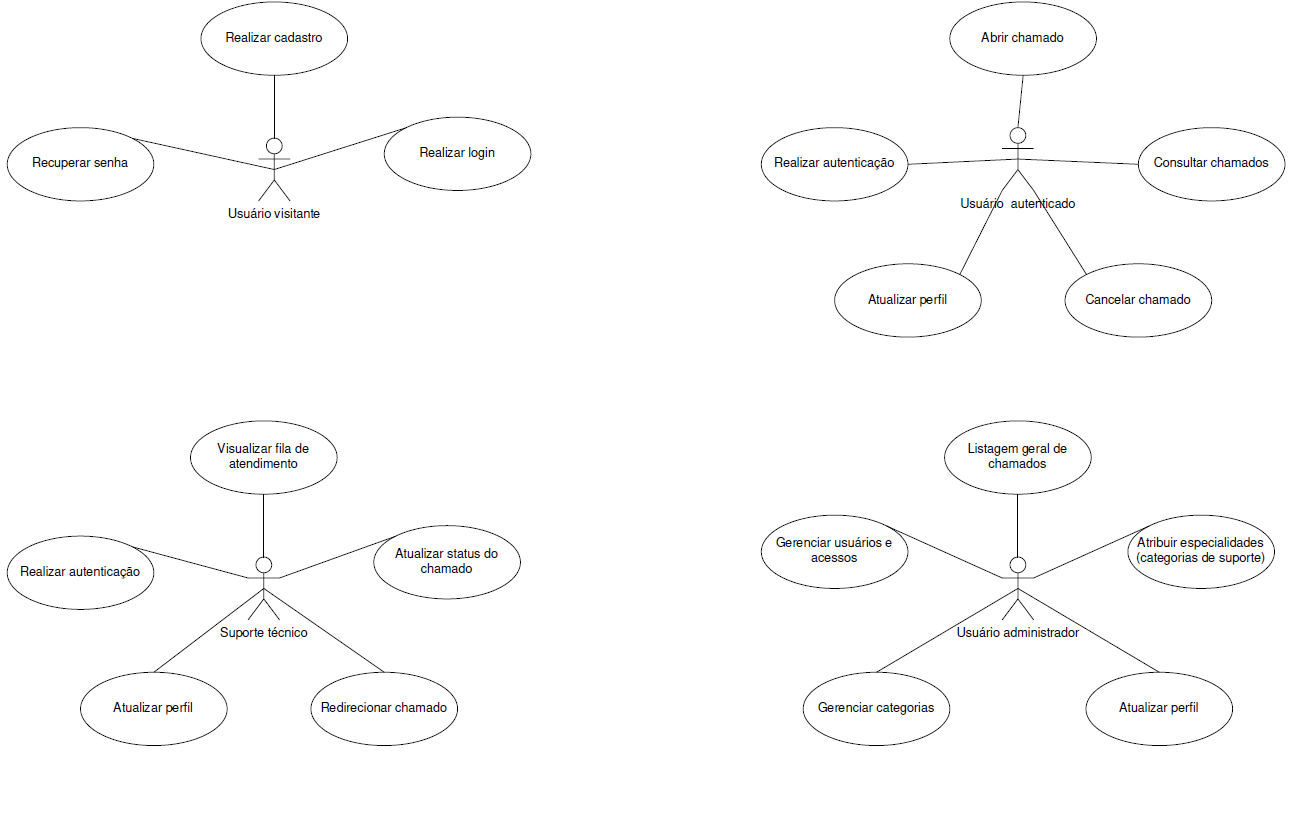
\includegraphics[width=0.8\textwidth]{Diagramas Projeto APO2/diagrama casos de uso.png}
    \caption{Diagrama de Casos de Uso do Sistema Help Desk.}
    \label{fig:casos-de-uso}
\end{figure}

\begin{figure}[htbp]
    \centering
    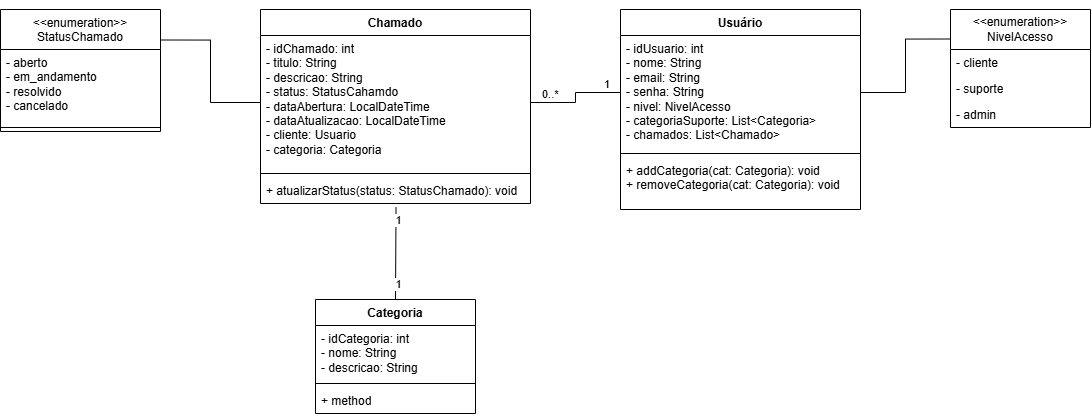
\includegraphics[width=0.8\textwidth]{Diagramas Projeto APO2/diagrama de classes apo2.drawio.png}
    \caption{Diagrama de Classes do Sistema Help Desk.}
    \label{fig:casos-de-uso}
\end{figure}

\begin{figure}[htbp]
    \centering
    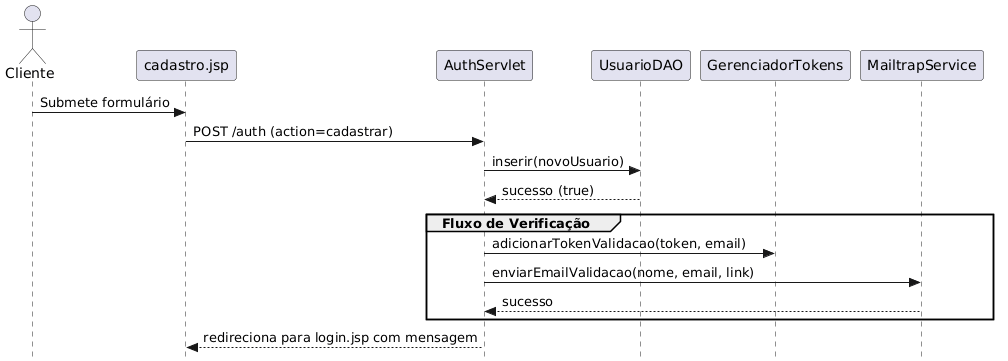
\includegraphics[width=0.8\textwidth]{Diagramas Projeto APO2/diagrama de sequencias - cadastro e verificação de email.png}
    \caption{Diagrama de Sequências do Cadastro do Sistema Help Desk.}
    \label{fig:casos-de-uso}
\end{figure}

\begin{figure}[htbp]
    \centering
    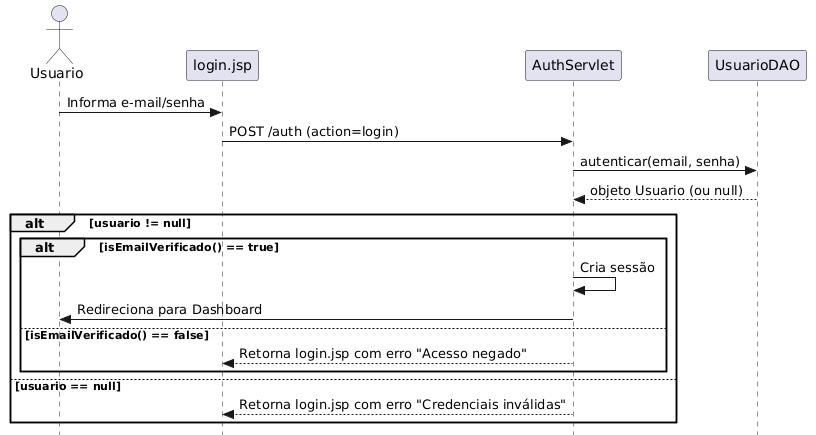
\includegraphics[width=0.8\textwidth]{Diagramas Projeto APO2/diagrama de sequencias - login e verificação.png}
    \caption{Diagrama de Sequências do login do Sistema Help Desk.}
    \label{fig:casos-de-uso}
\end{figure}

\begin{figure}[htbp]
    \centering
    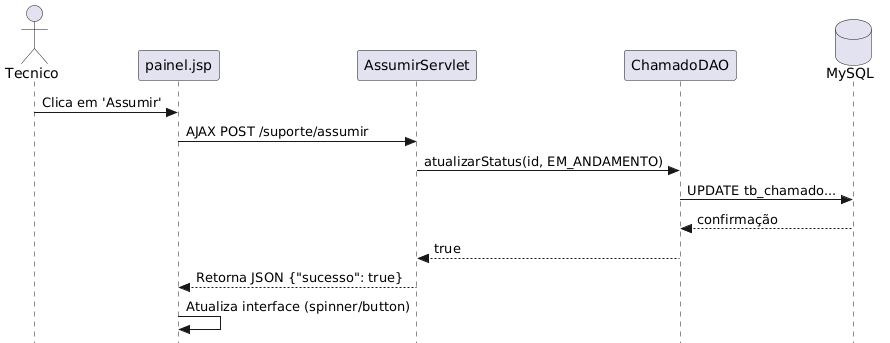
\includegraphics[width=0.8\textwidth]{Diagramas Projeto APO2/diagrama de sequencias - assumir chamado.png}
    \caption{Diagrama de Sequências UC: Assumir chamado}
    \label{fig:casos-de-uso}
\end{figure}

\begin{figure}[htbp]
    \centering
    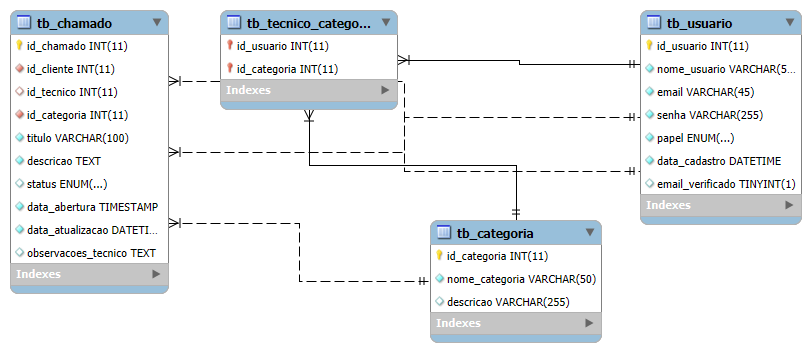
\includegraphics[width=0.8\textwidth]{Diagramas Projeto APO2/diagrama entidade e relacionamento.png}
    \caption{Diagrama de Entidade-Relacionamento}
    \label{fig:casos-de-uso}
\end{figure}

\end{document}

